\documentclass[tikz,border=3mm]{standalone}
\usepackage{pgfplots}
\pgfplotsset{compat=1.17}
\usepgfplotslibrary{groupplots}
\usetikzlibrary{arrows.meta,positioning,fit,shapes.geometric,calc,backgrounds}
\begin{document}

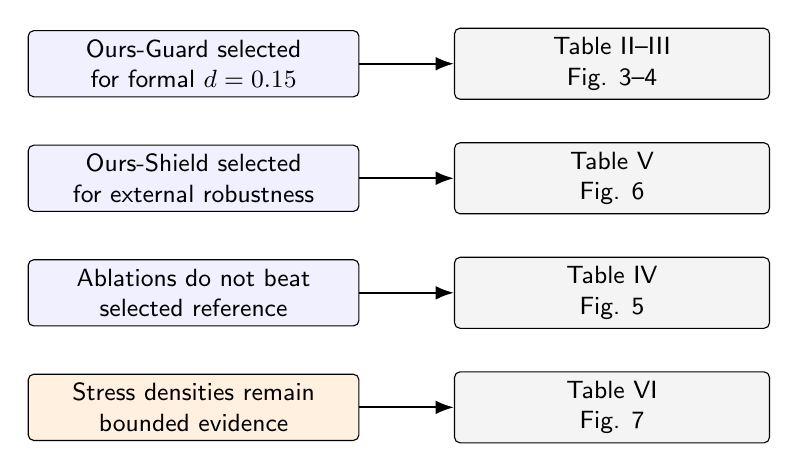
\begin{tikzpicture}[font=\sffamily\small, >=Latex, node distance=6mm and 12mm,
claim/.style={draw, rounded corners=2pt, fill=blue!6, align=center, minimum width=42mm, minimum height=8mm},
ev/.style={draw, rounded corners=2pt, fill=gray!9, align=center, minimum width=40mm, minimum height=8mm},
warn/.style={draw, rounded corners=2pt, fill=orange!12, align=center, minimum width=42mm, minimum height=8mm}]
\node[claim] (c1) {Ours-Guard selected\\for formal $d=0.15$};
\node[claim, below=of c1] (c2) {Ours-Shield selected\\for external robustness};
\node[claim, below=of c2] (c3) {Ablations do not beat\\selected reference};
\node[warn, below=of c3] (c4) {Stress densities remain\\bounded evidence};
\node[ev, right=of c1] (e1) {Table II--III\\Fig. 3--4};
\node[ev, right=of c2] (e2) {Table V\\Fig. 6};
\node[ev, right=of c3] (e3) {Table IV\\Fig. 5};
\node[ev, right=of c4] (e4) {Table VI\\Fig. 7};
\draw[->, thick] (c1)--(e1); \draw[->, thick] (c2)--(e2); \draw[->, thick] (c3)--(e3); \draw[->, thick] (c4)--(e4);
\end{tikzpicture}

\end{document}
